In this section, brief information about the methods and technologies used by Mooncascade's Android team while developing Android applications are presented. Sharing information about these methods and technologies at the baseline level is important for this study because qualitative and quantitative evaluations of their impact on maintainability and obtaining results on these effects are the primary purpose of this study.

First of all, the team uses Kotlin programming language for Android development. It is believed that the use of Kotlin can improve code quality, readability, and productivity \cite{44}. It is also the supported programming language by Google \cite{43}. For the same reasons the team prefers Kotlin over Java. Also, the team tries to adapt the Clean Code and SOLID principles to their daily programming tasks. Clean Code principles are believed to be to improve the readability and understandability of the code \cite{46}. Also, the application of SOLID principles facilitates the separation of concerns and improves code quality \cite{26}. The team applies these principles for these reasons and tries to maximize their application by code reviews.

When it comes to the architecture of Android application, the team prefers Clean Architecture\footnote{\url{https://blog.cleancoder.com/uncle-bob/2012/08/13/the-clean-architecture.html}}. Clean Architecture provides a high level of separation of concerns \cite{56} and facilitates changing third-party dependencies and implementation details of the software systems that it is used on. Also, it helps to modify the different layers of the application without affecting the business logic. Thus, it makes Android applications easy to understand, modify and test \cite{47}. The team also uses Model-View-View Model (MVVM) design pattern to present data and applies this design pattern with the help of tools provided by the Android Architecture Components framework published by Google's Android team\footnote{\url{https://developer.android.com/topic/libraries/architecture}\label{ft:arch-components}}. With the increase of the scale and the complexity of Android applications, a proper design pattern for the presentation of the data became essential for Android applications to achieve high cohesion and low coupling. Such design patterns enable the different degrees of separation for data, logic and view concerns. Also, an important characteristic for an efficient design pattern is eliminating the bidirectional dependency of views and view models. Thus decoupling of data and view becomes possible, and an important software design objective of high cohesion and low coupling is achieved. The MVVM design pattern provides these requirements for Android applications \cite{48}.

The team also uses some third-party Android and Java/Kotlin libraries to develop Android applications. Although such libraries are not a must when developing Android applications, the use of some of them saves Android developers a lot of time and effort. However, the team tends to reduce the use of third-party libraries as much as possible and prefers to use raw solutions whenever feasible. Community support, up-to-dateness, reliability and long-term maintainability criteria are considered when selecting the third-party libraries used. RxJava\footnote{\url{https://github.com/ReactiveX/RxJava}}, Dagger 2\footnote{\url{https://dagger.dev/}}, Retrofit\footnote{\url{https://github.com/square/retrofit}}, Apollo\footnote{\url{https://www.apollographql.com/docs/android/}} and Android Architecture Components$^{\ref{ft:arch-components}}$ are the most prominent libraries/frameworks and have the most impact on concepts such as Android application architecture and maintainability. RxJava is a library for designing asynchronous and event-based software applications by using observable sequences. Dagger is a static, compile-time framework used for dependency injection and it can be used by Java, Kotlin, and Android based applications. Retrofit is used to integrate REST-based back-end systems to Android applications, while Apollo is used for the integration of GraphQL based back-end systems. Lastly, Android Architecture Components are a set of libraries that facilitate designing robust, testable, and maintainable apps.

Lastly, in a related study, it is seen that the results obtained from Android practitioners are similar to the choices of Mooncascade Android team \cite{14}.
\begin{figure}[ht!]
    \centering
    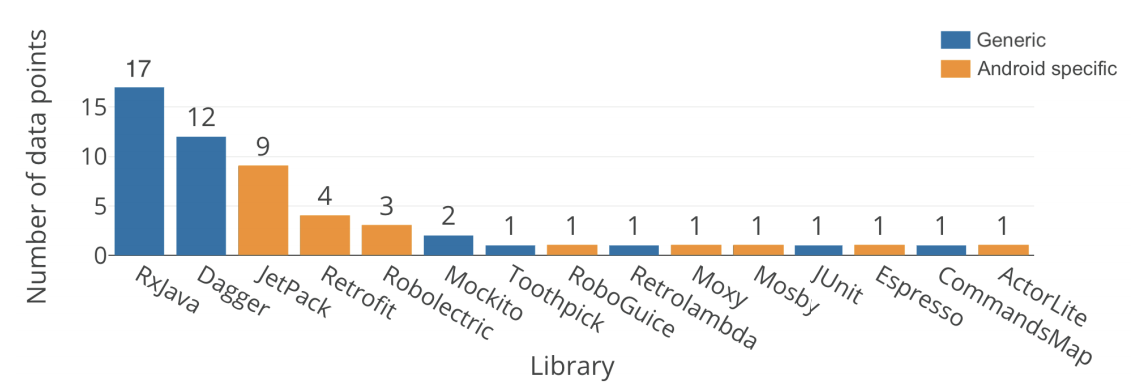
\includegraphics[scale=0.7]{figures/android-libraries.png}
    \caption{Developer tendencies for Android app architecture \protect\cite{14}}
    \label{fig:android-libraries}
\end{figure}
\FloatBarrier

Particularly, the interest of the participants in technologies such as RxJava, Dagger 2, Jetpack and Retrofit can be seen in this study. However, while making a correlation between the mentioned study, which was conducted two years ago, and the preferences of the case company, the rapidly changing nature of the Android ecosystem and changing trends should be taken into account.